% neginhib cogsci submission


\documentclass[10pt,letterpaper]{article}

\usepackage[
  breaklinks=true,
  bookmarks=false,
  pdfpagelabels=false,
  hyperfootnotes=false,
  hyperindex=false,
  pageanchor=false,
]{hyperref}

\makeatletter
\let\saved@hyper@linkurl\hyper@linkurl
%\let\saved@hyper@linkfile\hyper@linkfile
\let\saved@hyper@link@\hyper@link@
\AtBeginDocument{%
  % Since the whole document is affected, only the \begin part of
  % environment `NoHyper' is needed.
  \NoHyper
  \let\hyper@linkurl\saved@hyper@linkurl % needed by \url
  %\let\hyper@linkfile\saved@hyper@linkfile % needed by \href{<file>}
  \let\hyper@link@\saved@hyper@link@ % needed by \href{<url>}
}
\makeatother


\usepackage{cogsci}
\usepackage{pslatex}
\usepackage{apacite}
\usepackage{graphicx}

\usepackage{color}
 \newcommand{\denote}[1]{\mbox{ $[\![ #1 ]\!]$}}
 \definecolor{Red}{RGB}{255,0,0}
\newcommand{\red}[1]{\textcolor{Red}{#1}}
\definecolor{Green}{RGB}{10,200,100}
\definecolor{Blue}{RGB}{10,100,200}
\definecolor{DarkOrange}{RGB}{255,100,50}
\definecolor{Purple}{RGB}{160,0,160}
\newcommand{\ejy}[1]{\textcolor{Blue}{[ejy: #1]}}
\newcommand{\aen}[1]{\textcolor{DarkOrange}{[aen: #1]}}
\newcommand{\gabe}[1]{\textcolor{Green}{[gabe: #1]}}
\newcommand{\mcf}[1]{\textcolor{Purple}{[mcf: #1]}}

\title{Distinguishing processing difficulties in inhibition, implicature, and negation}

\author{{\large \bf Ann E. Nordmeyer} \\
 \texttt{anordmey@stanford.edu} \\
 Department of Psychology \\
 Stanford University
 \And {\large \bf Erica J. Yoon} \\
 \texttt{ejyoon@stanford.edu} \\
 Department of Psychology \\
 Stanford University
 \And {\large \bf Michael C. Frank} \\
 \texttt{mcfrank@stanford.edu} \\
 Department of Psychology \\
 Stanford University}

\begin{document}

\maketitle


\begin{abstract}

Despite their considerable communicative abilities, young children often have difficulty interpreting complex linguistic structures in context. Two examples of this phenomenon are negation and pragmatic implicature, both of which pose sometimes surprising difficulties for preschoolers. Both of these structures require children to resist a more salient alternative interpretation; since executive function abilities develop extensively during childhood, perhaps failures are due to problems in inhibition. To test this hypothesis, we designed speeded tasks to measure inhibitory control, negation, and implicature comprehension in children and adults. Using standard analyses as well as drift diffusion models, we found different patterns of processing on all three tasks, and no support for the hypothesis that inhibitory control per se is playing a role in either adults' or children's negation or implicature processing. Instead, our analyses reveal qualitatively different developmental trajectories for each task, suggesting task-specific factors driving these changes.

\textbf{Keywords:}
Inhibitory control; negation; implicature; drift diffusion model; cognitive development; pragmatics
\end{abstract}


\section{Introduction}

%
%\ejy{I liked the intro because it's a nice summary of what we're trying to do (so maybe it'll make a good beginning of our abstract) but I wonder if this is still confusing for some naive readers who have no idea what ``linguistic constructions'' we are talking about. I'm going to try something else here (now that I look at it, maybe it won't work... see what you think and feel free to change it back!)}
%
%\aen{I changed it back, because I think it's important to introduce both tasks (and our overarching hypothesis) in the first sentence. I agree with your overall point, though, and it's something I've been struggling with in this intro because it's hard to introduce so many complicated phenomena so succinctly! I tried to make it a little clearer what we're talking about here, but I don't know how if this is much better}

By ages 3--4, children are often quite proficient at general communication, using language to tell stories, coordinate actions, and generally navigate the social world \cite{clark2009}. Despite this proficiency, the same children often fail laboratory language processing tasks that test important but complex linguistic constructions. For example, in tests of negative sentence comprehension, children will often struggle to identify a character who has ``no apples,'' instead choosing the character who \emph{does} have apples \cite{nordmeyer2014b}. And while adults easily make the ad-hoc pragmatic implicature that ``My plate has a carrot'' refers to a plate with \emph{just} a carrot (rather than a plate with a carrot and a banana), children often fail \cite<see example stimuli in Figure \ref{fig:stimuli};>{yoonchildren}.

Children's difficulties with these tasks are surprising in light of their other abilities in each domain. Children spontaneously produce negation before their second birthday in both natural \cite{bloom1970, pea1980} and experimental contexts \cite{pea1982}. Yet children as old as four years consistently fail tests of negation comprehension \cite<e.g.>{kim1985, nordmeyer2014b}. And children demonstrate an understanding of pragmatic principles by age three \cite{clark2009}, adjusting the informativeness of their own expressions depending on the difficulty of referent disambiguation \cite{matthews2006} and the extent of listeners' knowledge \cite{matthews2012}. Yet they stuggle to make ad-hoc implicatures before age four \cite{yoonchildren,stiller2015} and scalar implicatures with quantifiers beyond age five \cite{huang2009}.

% Although these two examples, negation and pragmatic implicatures, come from very different linguistic phenomena, comprehension on both tests requires children to resist choosing a more salient (but incorrect) alternative. Correct comprehension of negation in the situation described above requires avoiding choosing the more interesting character (the one who has apples), whose image also directly matches the target noun. And correct comprehension in the ad-hoc pragmatic implicature task requires avoiding choosing the more enticing choice as well (the plate with more fruit). Could poor inhibitory control account for children's difficulty on both of these tasks?

Why do children struggle on negation and implicature when production data and past experiments suggest that they have the requisite linguistic abilities? In both of these examples, children's failures might occur not because they lack linguistic understanding, but because the incorrect choice is more salient or perceptually interesting. When a child is asked to ``find the boy with no apples,'' she must look \emph{away} from the character who is holding the labeled objects, and look at some other, unlabeled object instead. Similarly, to demonstrate comprehension of ``my plate has a carrot," children must look away from the more visually salient plate (the one with two objects instead of one). In both of these cases, poor executive function might explain children's difficulty selecting the correct response on these comprehension tasks.

Executive function is a construct that encompasses a wide variety of different functions including response inhibition, task-shifting, and working memory \cite{miyake2000}. These abilities change dramatically during early childhood \cite{diamond1996,davidson2006}, especially during the period of interest (very roughly, ages 3--5), making them a possible candidate factor underlying changes in language processing. The specific executive function construct most relevant to negation and implicature is response inhibition, because classic tests of this construct require participants to override a prepotent response. Participants who react quickly often make the wrong choice, and correct choices are typically slower. The presence of these sorts of speed-accuracy tradeoffs in language comprehension data might be a signal of inhibitory issues, but speed-accuracy tradeoffs can be difficult to understand with traditional analyses, which examine reaction time and accuracy separately.


\begin{figure*}[t!]
\begin{centering}
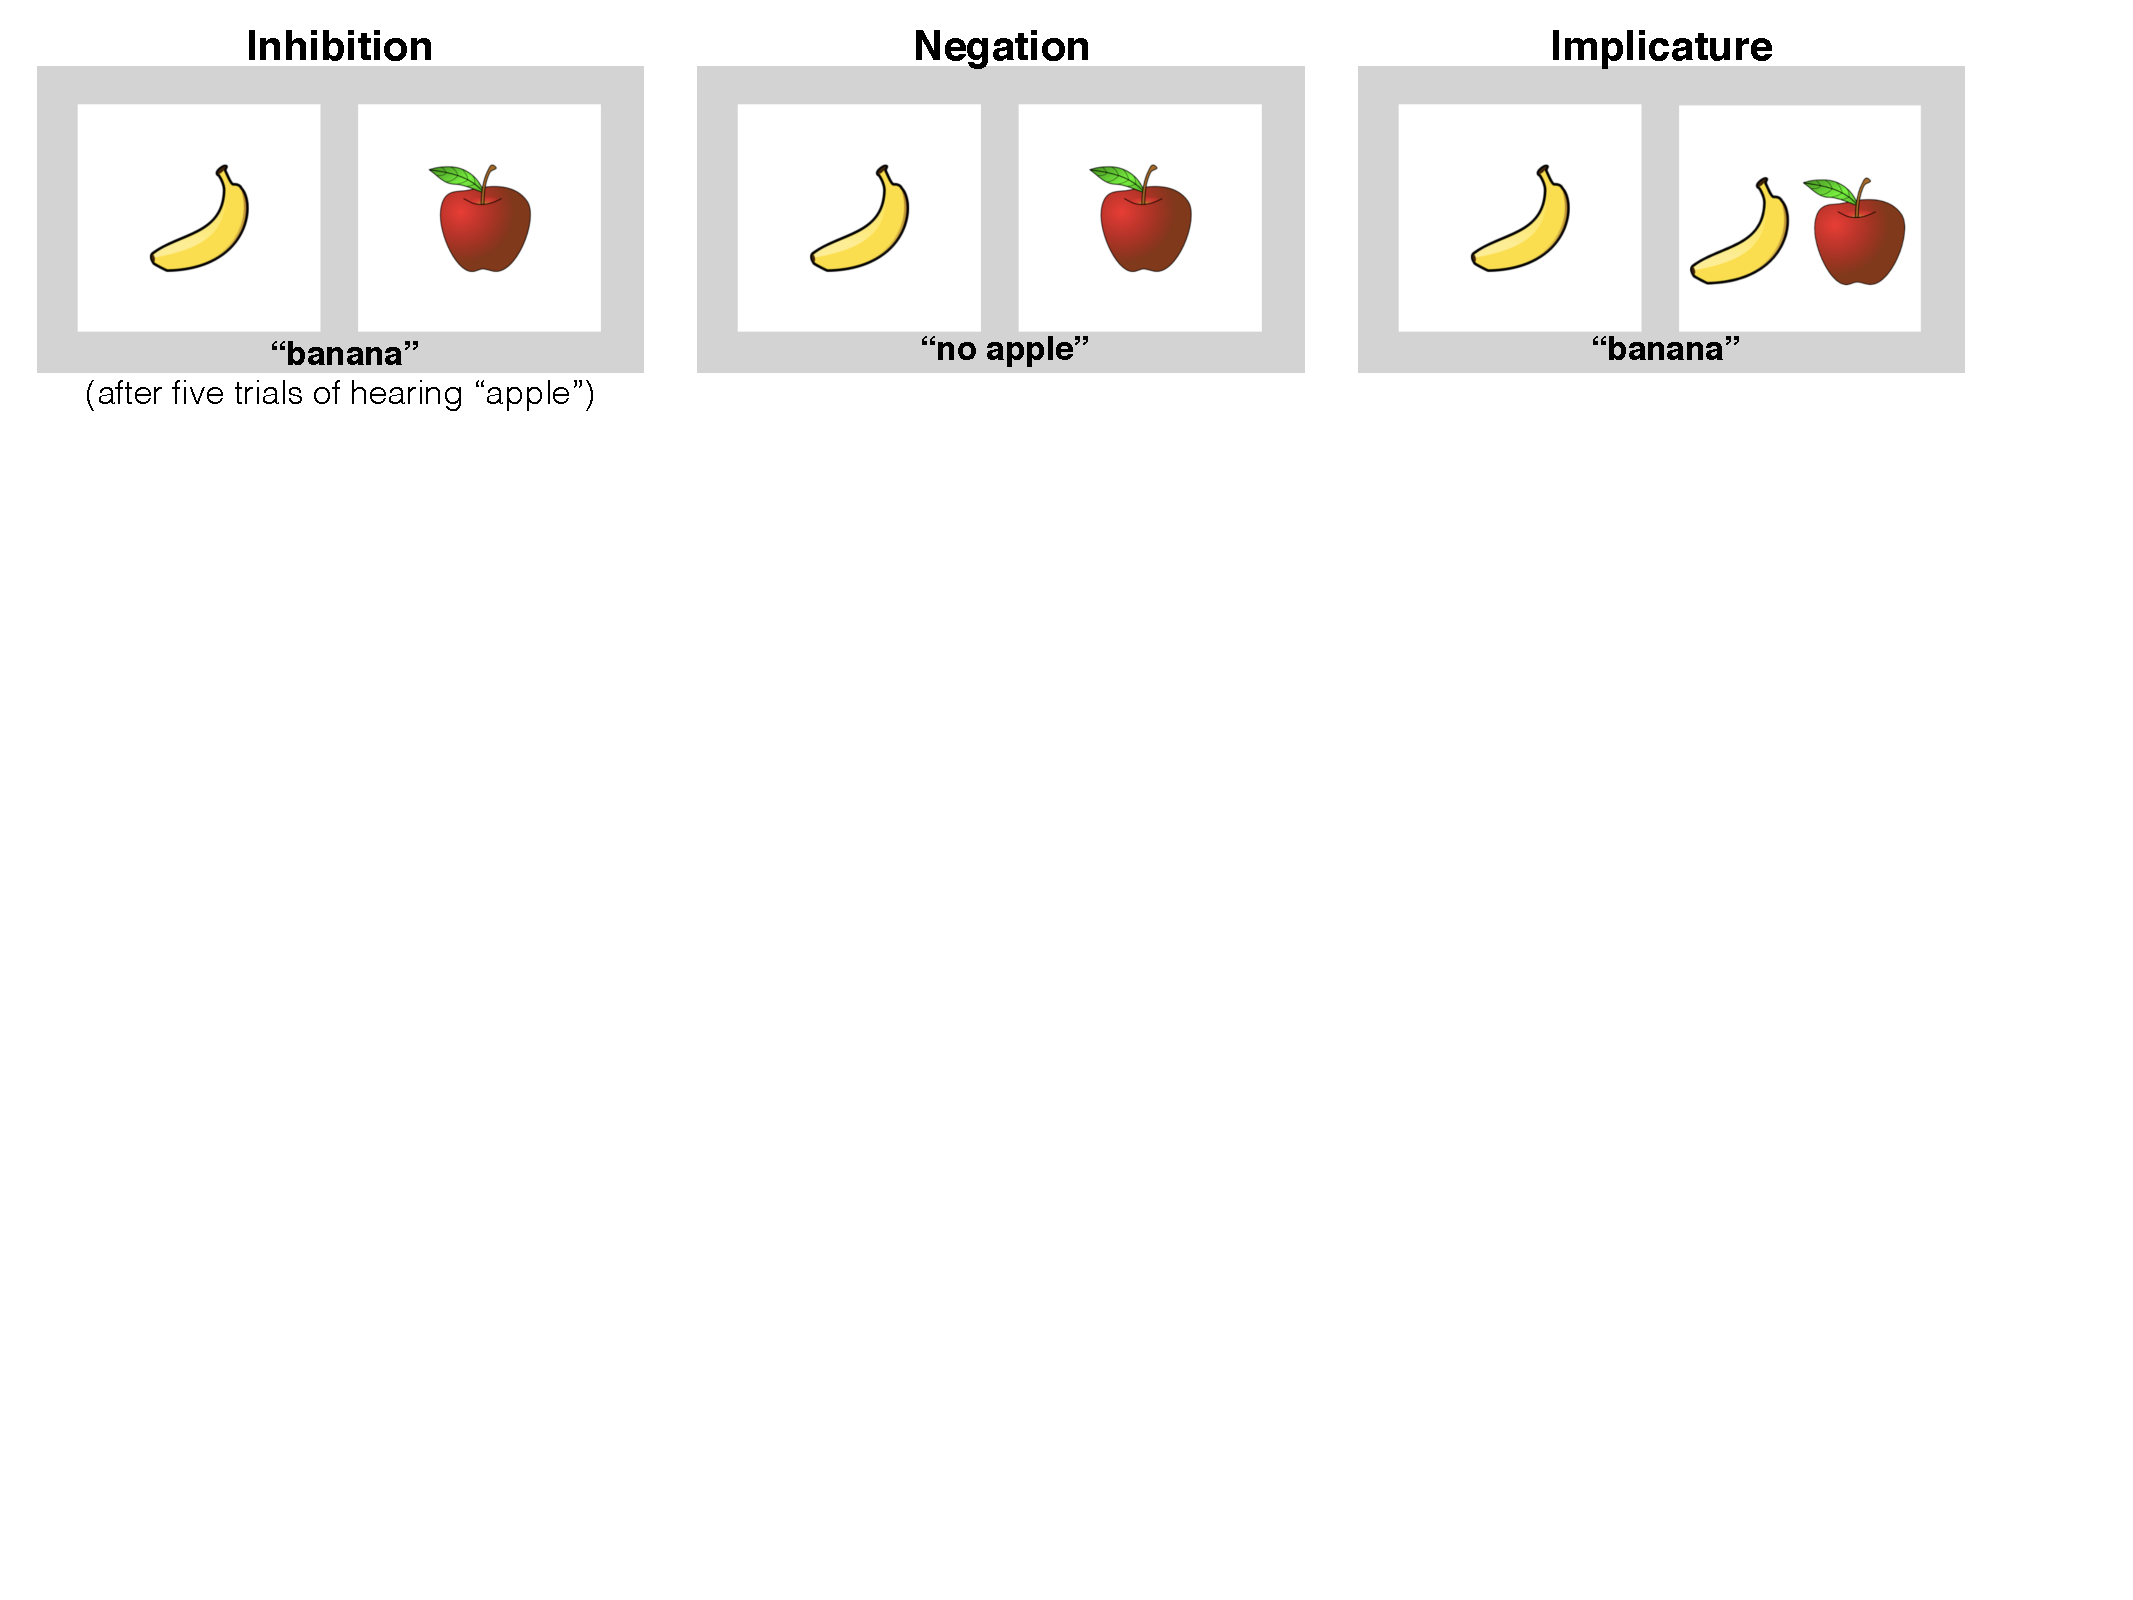
\includegraphics[width=\textwidth]{figures/stimuli.pdf}
\caption{\label{fig:stimuli} Example stimuli from each condition. Words identifying the target picture (left in each panel) are given at the bottom.}
\end{centering}
\end{figure*}

Drift diffusion models (DDMs) are an important tool for addressing the speed-accuracy tradeoff that often arises in response inhibition tasks. DDMs \cite<e.g.>{ratcliff1978theory} use both accuracy and reaction time as measures of the decision making process in simple two-alternative forced choice paradigms. The model can be imagined as a noisy accumulation of evidence over time, resulting in an eventual correct or incorrect choice when the accumulated evidence reaches a predetermined decision ``boundary.'' The model produces four key parameters: boundary separation (the amount of evidence needed to reach a positive decision), bias (to what extent is the decision process biased towards one decision or another), non-decision time (the time needed to encode basic information about the stimuli, before embarking on the decision process), and drift rate (the rate at which evidence is accumulated). Past work has shown that children typically have longer non-decision times, higher separation boundaries, and slower drift rates, suggesting that children require more time to process stimuli, more information to make a decision, and take longer to accumulate evidence compared to adults \cite{ratcliff2012}.

In the current work, we test the hypothesis that changes in response inhibition underly developmental changes in children's processing of negation and implicature. We use a simple design with three separate subtasks to test adults' and children's inhibitory control, negation comprehension, and implicature comprehension. In order to explore how children's language processing changes across development, we collected data from 4--6-year-olds, as well as adults. Despite the fact that the three tasks contained almost identical visual and auditory stimuli, results of conventional and DDM analyses suggest distinct patterns of information processing and developmental change across the three tasks. This suggests that, contrary to our hypothesis, children's undeveloped inhibitory control cannot entirely explain their difficulty with negation and pragmatic implicatures, and children's development of negation and implicature appear to follow different developmental trajectories throughout early childhood.


\section{Method}

We created three simple ``find the picture'' tasks (stimuli pictured in Figure \ref{fig:stimuli}) to test inhibitory control, negation, and implicature in adults and children. Our initial version of this task was implemented on an iPad tablet (and results were similar), but in this version we used a computer to facilitate shorter reaction times and increase comparability between the children and an online sample of adults (who used a computer).

% In pilot work, we used a classic ``find the picture'' comprehension task to explore whether 4-year-old children's difficulty processing implicatures and negation might be due to poor inhibitory control. Our hypothesis was that undeveloped inhibitory control could lead children to quickly choose the more salient incorrect choice rather than selecting the answer they know to be correct. Although we did not find any correlation between children's inhibitory control processing and their negation or implicature processing, we found that this simple comprehension task was even more challenging for 4-year-olds than our past work has indicated, with 4-year-olds barely exceeding chance performance on negation and implicature trials. Surprisingly, we found no reaction time differences between 4-year-olds responses to negation/implicature trials and control trials. In our extension of this pilot data we modeled children's responses using the drift diffusion model, which can help us understand the process that leads children to make so many errors on these tasks. \aen{Erica suggested cutting some of these details out to save space; I also think some of these details should go in the results section (e.g. to motivate why we did the DDM).}

\subsection{Participants}

We invited parents and children at the Children's Discovery Museum in San Jose, CA to play a computer game. Ten children were excluded from analysis because their parents indicated that they heard English at home 50\% of the time or less. An additional 24 children were excluded from analysis for failing to complete at least half of the trials in each task. These exclusions resulted in a final sample of 22 4-year-olds (mean age 4;7), 19 5-year-olds (mean age 5;5), and 25 6-year-olds (mean age 6;5). We also recruited adult participants on Amazon Mechanical Turk to play the computer version of the task. Two adults were excluded for failing to complete at least half of the trials, resulting in a final sample of 48.

\subsection{Stimuli and design}

The experiment consisted of three tasks: inhibition, negation, and implicature. In each trial in all three tasks, there were two images side by side on the screen. A pre-recorded voice said one or two words, and participants' task was to select the correct referent as soon as they could. We used words (instead of full sentences) both to keep linguistic stimuli as similar as possible across the three tasks and to keep trials very short, allowing us to collect many trials per participant (a requirement of the planned DDM analyses). On each task, participants were instructed to select the corresponding picture as quickly and accurately as possible.  

For the inhibition task, in a set of 6--8 trials, the same two pictures appeared side by side (e.g., a picture of a banana and a picture of a apple). The target picture appeared on either the left or the right side, with target side randomized across all trials. For the first 5--7 trials (control trials), one of the two objects was named (e.g., ``apple''), then on the last trial (target trials), the other object was named (``banana'').
% Participants were predicted to become increasingly accustomed to choosing the carrot in control trials. Then in the target trial, when they need to switch and choose the banana, accuracy rate was predicted to fall due to the inhibitory demand.
Children saw a total of 12 sets of trials, and adults saw 24 sets.

For the negation task, the referents were named with or without negation. For example, given two pictures of banana and apple respectively, to refer to the banana the recorded voice said ``banana'' (positive trials, the control for this task) or ``no apple'' (negative trials, the target for this task). Children saw 60 trials, and adults saw 120 trials.

For the implicature task, in each trial there was a picture with one object (e.g., banana) and another picture with the same object as well as another (e.g., banana and apple). In control trials, the unique object was named (``apple'') and in target trials, the common object was named (``banana''), implying ``banana \emph{but not apple}'' (an ad-hoc implicature). Children saw 60 trials, and adults saw 120 trials.

\begin{figure*}[t!]
\begin{center}
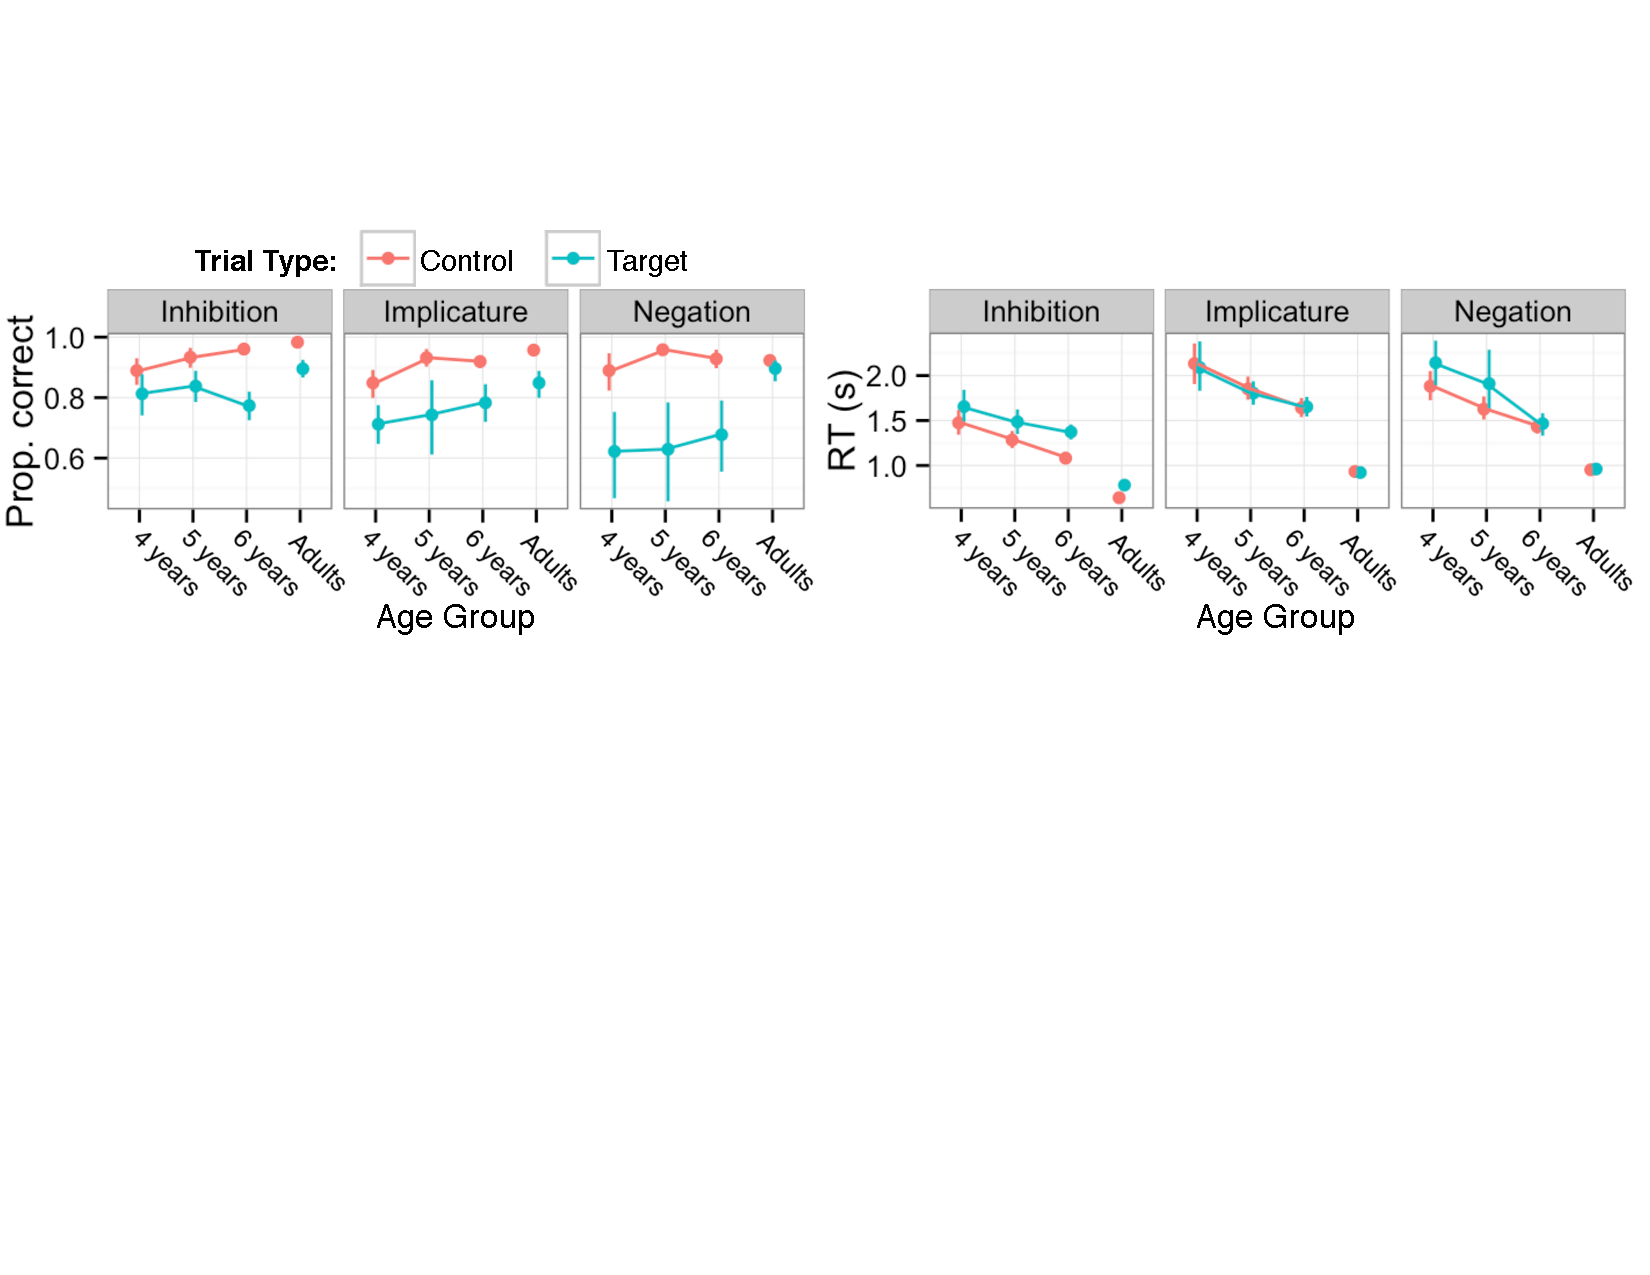
\includegraphics[width=\textwidth]{figures/correct_RT_v2.pdf}
\caption{\label{fig:traditional} Adults' and children's mean proportion correct responses (left) and reaction time (right) for target and control trials across the three tasks. Control trials are shown in red, target trials are shown in turquoise. Error bars show 95\% confidence intervals. }
\end{center}
\end{figure*}

\subsection{Procedure}

An experimenter first explained the task to children, who then went through two practice trials, where they were asked to select an obvious, unambiguous referent (e.g., ``cow'' as opposed to ``rabbit''). Children selected the picture on the left side of the screen by pressing the `z' key and selected by picture on the right side of the screen by pressing the `/' key; both keys were covered by blue stickers to help children find them. Then they went through the three tasks in a randomized order. Afterwards, the experimenter gave them a sticker as a gift. Adults played the same game without practice trials.
% Instructions indicated that participants should select the picture on the right by pressing the `p' key and select the picture on the left by pressing the `q' key.



\subsection{Analysis and preprocessing}

Because some children responded immediately without listening to the entire word and some children took an exceedingly long time to respond to some trials, we made a decision to remove any trials with reaction times less than 200 milliseconds from the word onset, and longer than 15 seconds from the word onset.\footnote{Although this decision was made post-hoc based on some unexpectedly short and long reaction times, the decision did not affect the key findings we present in this paper.} After these initial exclusions, we followed our initial planned analysis by removing RTs outside of three standard deviations from the log-transformed mean.

We fit diffusion models separately to each individual participant's data using the RWiener package,\footnote{All analyses described in this paper were conducted using R version 3.2.1} using the Nelder-Mead method to estimate optimal parameter values. We estimated parameters separately for each trial type (target vs. control) within each task, and calculated the mean and 95\% C.I. across all participants within each age group (4-year-olds, 5-year-olds, 6-year-olds, and adults), and removed participants with any parameter value outside of 3 standard deviations from the mean for that parameter within each game.  

All regression results are reported based on linear (for RT and DDM parameters) or logistic (for accuracy) mixed effect models, fit using \texttt{lme4} with the maximal convergent random effect structure. Models of RT were fit using log-transformed RTs.

 % We then used these parameter estimates to produce visualizations of the average decision process for each trial type across each game and age group (see Figures \ref{fig:ddm}).

\section{Results and Discussion}

This experiment yielded a large data set that affords many analyses.  Participants' accuracy and reaction times are shown in Figure \ref{fig:traditional}; DDM fits are shown in Figure \ref{fig:ddm}. We organize the results reported here around those findings that speak most directly to our question of interest.  First we use traditional accuracy and reaction time measures to examine whether individual performance on the inhibition task is correlated with individual performance on the implicature and negation tasks. We then use the drift diffusion model to explore differences in processing across the three tasks, and examine the development of children's processing in each task.  Raw data are available at \href{https://github.com/anordmey/cogsci16}{\nolinkurl{https://github.com/anordmey/cogsci16}}, and a fuller set of analyses can be viewed at \href{http://anordmey.github.io/cogsci16/analysis/neginhib_cogsci16.html}{\nolinkurl{http://anordmey.github.io/cogsci16/analysis/neginhib_cogsci16.html}}.

% \subsection{Accuracy and Reaction Time}

\subsection{Inhibition task performance was not correlated with negation or implicature performance}

% Across all three games, participants were more accurate on control trials (i.e., repeated trials in the inhibition game, unambiguous trials in the implicature game, and positive trials in the negation game) compared to target trials (i.e., switch trials in the inhibition game, implicature trials in the implicature game, and negative trials in the negation tame). This difference in accuracy between control and target trials was true across all age groups for the inhibition and implicature games (main effect of trial type, inhibition game: $\beta = -2.10$, $p< .001$; implicature game: $\beta = -1.15$, $p< .001$). For the negation game, this difference was present for children but not adults (trial type x age group interaction: $\beta = -1.98$, $p< .001$). Both children and adults also took slightly longer to respond correctly to target trials compared to control trials on the inhibition game (main effect of trial type in linear mixed-effects model, inhibition game: $\beta = 0.14$, $p< .001$), but there was no main effect of trial type in the negation or implicature games.

Our key hypothesis was that successful performance on the negation and implicature tasks requires inhibitory control, and hence performance on negation and implicature should be correlated with performance on inhibition. To test this hypothesis, we calculated standardized difference scores between target trials and control trials for each participant on each task, using both accuracy and RT. For accuracy, we found no significant correlations between individual accuracy on the inhibition task and the implicature task for adults ($r = .21$, $p = .16$, 95\% CI [-0.08, 0.46]) or kids ($r = -.09$, $p = .49$, 95\% CI [-0.32, 0.16]), nor between individual accuracy on the inhibition task and the negation task for adults ($r = -.11$, $p = .46$, 95\% CI [-0.38, 0.18]) or kids ($r = -.08$, $p = .51$, 95\% CI [-0.16, 0.32]). For RT, there was similarly no relationship between individual RT on the inhibition task and the implicature task for adults ($r = -.004$, $p = .98$, 95\% CI [-0.29, 0.28) or kids ($r = .20$, $p = .11$, 95\% CI [-0.04, 0.42]), nor between individual RT on the inhibition task and the negation task for adults ($r = .17$, $p = .25$, 95\% CI [-0.12, 0.43]) or kids ($r = -.01$, $p = .92$, 95\% CI [-0.24, 0.26]). 

Consistent with past findings \cite<e.g.>{nordmeyer2014b, yoonchildren}, we found a great deal of individual variability in children's performance on these tasks, with 4- to 6-year-olds struggling especially on the implicature and negation tasks. Contrary to our hypothesis, however, performance on these two tasks was not correlated with performance on the inhibition task. One drawback to these traditional analyses is that they separate reaction time and accuracy, obscuring any potential interaction between the speed at which participants make a decision and the accuracy of their decision. In the next sections, we use the parameters of drift diffusion models to compare participants' decision-making processes.

\subsection{Adults show different decision processes for inhibition, implicature, and negation}

\begin{figure*}[t!]
\begin{center}
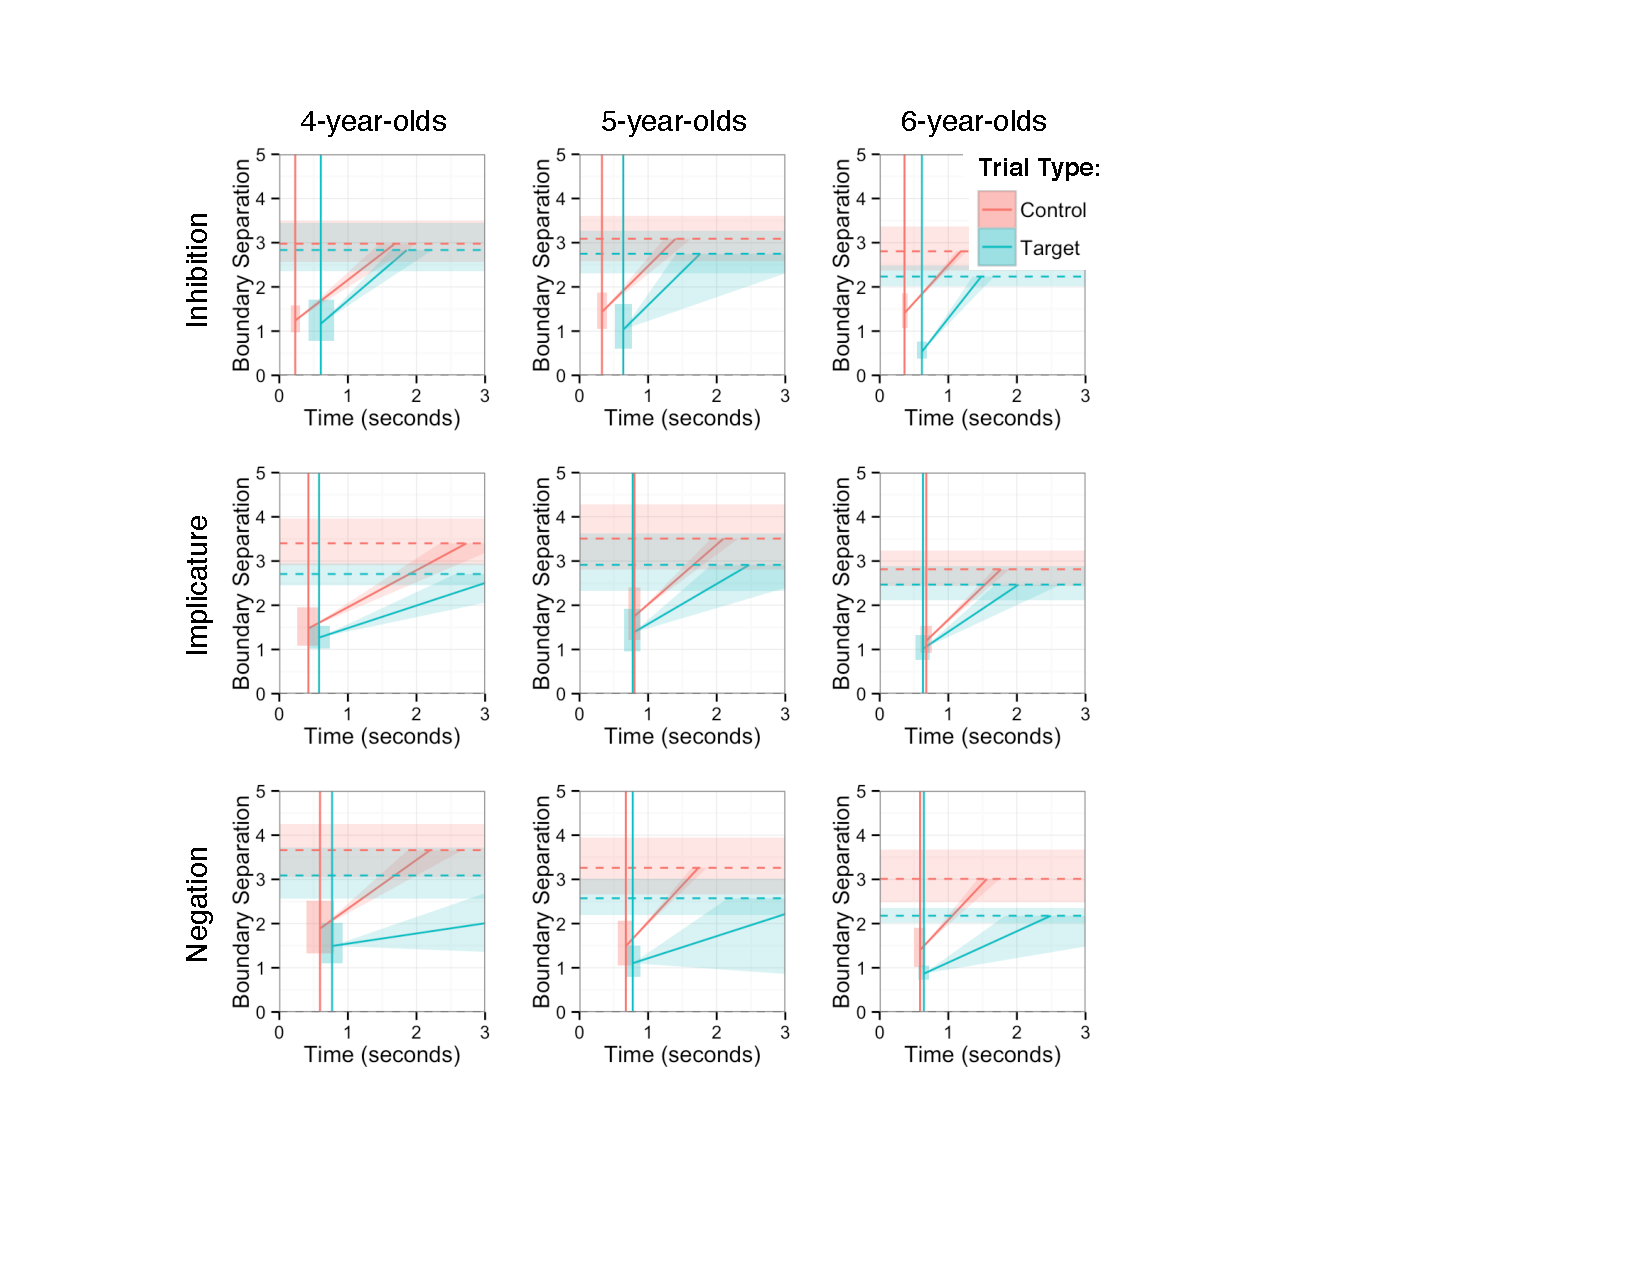
\includegraphics[width=\textwidth]{figures/ddm_vis.pdf}
\caption{\label{fig:ddm} Visualization of the drift diffusion process across the three tasks. The process for control trials is shown in pink, and the process for target trials is shown in green. The dotted black line at zero represents the threshold for making an incorrect decision, and horizontal colored lines represent the boundary separation parameter (i.e., the threshold for making a correct decision). Vertical colored lines represent the non-decision time parameter, and the slope of the decision process (angled line) represents the drift rate parameter. The point where the decision process crosses the non-decision line represents bias $\times$ boundary separation. Ribbons around all lines represent 95\% confidence intervals around each parameter.}
\end{center}
\end{figure*}

% First we explored similarities and differences in the decision process for adults across each of the three games (rightmost plots in
% ).
Despite the surface similarities of these tasks, adults' decision processes for control vs. target trials were different across the three tasks (Figure \ref{fig:ddm}, right panels). In the inhibition task, the most striking difference between control and target (inhibition) trials was the bias towards incorrect responses on target trials. The bias parameter was significantly lower for target trials compared to control ($t(43) = 4.92$, $p< .001$); target trials also had significantly longer non-decision times compared to control trials ($t(43) = -9.36$, $p< .001$). The bias effect is easily interpretable in the context of the task, because the repeated references to the control object were designed to create such a bias.

In the implicatures task, the most noticeable difference between control and target trials was the higher boundary separation but faster drift rate for control trials compared to target trials (boundary separation: $t(44) = 4.21$, $p< .001$; drift: $t(44) = 7.15$, $p< .001$). The slower drift rate for target trials in the implicatures task might have arisen due to their ambiguity (either picture is technically correct): Participants might have been slower to accumulate information to resolve this ambiguity. The fact that the boundary separation is higher for control trials in the implicatures task, combined with this slower drift rate, explains why reaction times do not differ between trial types on the implicatures task, despite lower accuracy for target trials.

Finally, in the negation task, there was no difference in parameters between positive and negative trials. For example, there was no significant difference between drift rates ($t(43) = 0.80$, $p = .43$). This was surprising in light of past work suggesting that adults take longer to respond to negative sentences compared to positive ones \cite{hclark1972}, especially in context-free tasks such as this one \cite{nordmeyer2014a}. One possibility is that the large number of repetitive trials, or the simplistic and child-friendly stimuli, made this task easier for adults.

% Next we turned to examining developmental change in children's decision processes, using the DDM to explore general developmental change in children's information processing as well as separate developmental trajectories for each of the three games.

\subsection{Information processing improves with age}

% First we examined overall changes in children's information processing, regardless of the task that children were engaged in.

Across all three tasks, children at all age groups had different parameter values than adults: higher boundary separation (4-year-olds: $\beta = 1.09$, $p <.001$; 5-year-olds: $\beta = 1.15$, $p <.001$; 6-year-olds: $\beta = .74$, $p <.001$) and longer non-decision times (4-year-olds, $\beta = .18$, $p = .09$; 5-year-olds: $\beta = .18$, $p <.001$; 6-year-olds: $\beta = .10$, $p <.001$), suggesting that children take longer to encode information and need more information to make a decision compared to adults. Children also had significantly slower drift rates compared to adults (4-year-olds: $\beta = -1.63$, $p <.001$; 5-year-olds $\beta = -1.22$, $p <.001$; 6-year-olds: $\beta = -1.13$, $p <.001$), suggesting that children acquire evidence more slowly than adults.
% These data replicate past findings from \citeA{ratcliff2012}, which found similar differences between adults and elementary-school aged children.

To explore whether these parameters changed significantly throughout these early years, we next focused just on children's data and analyzed age group as a continuous variable. This analysis revealed a significant increase in drift rate across these three years ($\beta = .25$, $p < .001$), as well as significant decreases in separation bias ($\beta = -.18$, $p < .01$) and non-decision time ($\beta = -.04$, $p < .05$). These findings indicate that the speed at which children accumulate evidence and the amount of information that children need to make a decision changes rapidly across early childhood.

\subsection{Children show different developmental trajectories for inhibition, implicature, and negation}

% Next we examined how children's decision processing changes for each of the three games across development.
In addition to the general developmental changes in drift rate, non decision time, and boundary separation described in the previous section, children's decision process for each task showed a distinct pattern of development from four to six years of age.

% \emph{Inhibition:}
In the inhibition task, 4-year-olds were \emph{less} likely to show a bias towards the incorrect trial compared to adults; this bias appears to get stronger by age 6. Linear models fit to individual parameter values for each task revealed a significant positive interaction between age group and trial type for four-year-olds' bias parameter ($\beta = .14$, $p< .05$), indicating that for four-year-olds the bias parameter for target trials in the inhibition task is higher compared to adult participants. There was no interaction between age group and trial type for five-year-olds ($\beta = .06$, $p = 37$) or six-year-olds ($\beta = -.06$, $p = .31$). These results collectively suggest that while four year olds are \emph{less} biased towards the incorrect response on target trials compared to adults, by age five children are becoming more biased towards the incorrect response on target trials.

In the implicature task, children's drift rates increased developmentally, but the increase in drift rate occurred primarily in control trials. This pattern led to an increasing difference in drift rates between control and target trials across development, driven primarily by an increase in control trial drift rate. Drift rates for target trials remain low even in adulthood, presumably due to the ambiguous nature of these trials. Confirming these findings, linear models fit to individual parameter values for each task resulted in significant positive interactions between age group and trial type at all ages (four-year-olds: $\beta = 0.63$, $p <.01$; five-year-olds: $\beta = 0.80$, $p <.01$; six-year-olds: $\beta = 0.49$, $p <.05$).

The negation task yielded the most striking difference between adults and children. Children had much lower drift rates for target trials compared to control trials. Drift rates on negation trials for four-year-olds were close to zero, suggesting a pattern of general uncertainty for young children on this task. The primary developmental change for this task was an increase in drift rate for target trials, with significant negative interactions between age group and trial type for four, five, and six-year-olds (4-year-olds, marginally significant: $\beta = -0.53$, $p = .07$; 5-year-olds: $\beta = -1.06$, $p <.001$); 6-year-olds ($\beta = -0.83$, $p < .01$).

% \ejy{should report on correlations between individual children's parameters somewhere? Or is that going to be in the markdown?} \aen{It is in the markdown, but I can add a sentence here mentioning it. I've been thinking about the individual parameter correlations though and it isn't even clear to me what our predictions would be about these correlations. Given that in the adult data we see such different patterns of processing across the three games, why would we even expect to see a relationship between e.g. kids drift rate on the inhibition game and kids drift rate on another game? That's why I ended up not talking about it here}

% Furthermore, the drift diffusion analysis yielded informative differences in the development of negation and implicature comprehension.

Although children struggled on both negation and implicature tasks, children's difficulty on the implicature task appeared to be due to general changes in information processing across development, as indicated by improvement primarily in the control trials of this task. In contrast, children's difficulty on the negation task appeared to be due to unexpectedly low drift rates for negation trials compared to control trials, a difference that disappeared in adulthood. \emph{Why} children appear to struggle so much on the comprehension of negative sentences, despite producing similar sentences at a much younger age, remains an open question.
% Contrary to our expectations, we found no evidence that children's difficulty on implicature and negation tasks was related to their performance on an inhibitory control task.


\section{General Discussion}

We created a set of three tasks to explore children's and adults' inhibitory control, implicature processing, and negation processing. Our experiment was designed to test the hypothesis that negation and implicature processing require inhibitory control, and that children's poor performance on these tasks is due to poor inhibitory control. Contrary to our hypothesis, we did not find any evidence of a relationship between performance on the inhibition task and performance on the negation or implicature tasks. Drift diffusion models revealed different patterns of processing on all three tasks, with no evidence that adults or children are biased towards the incorrect answer (as in the inhibition task) on implicature or negation tasks. Our analysis sheds light on the developmental trajectory of children's inhibitory control, negation processing, and pragmatic inference, suggesting that children's low performance on negation and implicature comprehension tasks may be caused by separate processing difficulties.

The current work used a unified procedure which allowed us to directly compare different linguistic and non-linguistic processes. The drift diffusion analysis revealed important findings in our data that could not have been found using traditional analyses of reaction time and accuracy. Although our three tasks were nearly identical in appearance---they used the same few trial images and labels and had the same basic instructions to select the correct picture---the decision process for adults to choose the correct picture was very different for each task. For example, the inhibition task was characterized by a bias towards the incorrect answer on target trials, while the implicatures task was characterized by slower drift rates for target trials.

Children's difficulty on the negation and implicature games appears to be due to slow accumulation of information on these tasks. Past work suggests that children typically have slower drift rates compared to adults \cite{ratcliff2012}, and our current work replicates that finding. In our tasks older children had faster drift rates compared to younger children on all tasks, but this developmental increase in drift rate occurred particularly for control trials on the implicature task and target trials on the negation task. The fact that children's drift rates for negation trials were significantly slower compared to adults suggests that children find it particularly difficult to process the relevant information about negation above and beyond a generally slower processing speed for children compared to adults. Whether the source of this difficulty is an undeveloped semantic understanding of truth-functional negation, or poor phonological processing---for example, perhaps some children simply miss the word ``no'' entirely---is a topic for future research.

A final novel aspect of this work is the use of the drift diffusion model with preschool children. Although some past work has explored children's information processing using the drift diffusion model \cite{ratcliff2012}, that work tested second graders at the youngest. Here we expand on that work by replicating their findings with a group of much younger children. Our success using the drift diffusion model with data from such young children opens doors for future work exploring the development of children's information processing.

\section{Acknowledgments}
%
We thank the parents, children, and staff at the San Jose Children's Discovery Museum. This work was supported by NSF grant BCS \#1456077.

%Bing Nursery School, CDM, Stephen Powell, Veronica, Rachel

\bibliographystyle{apacite}

\setlength{\bibleftmargin}{.125in}
\setlength{\bibindent}{-\bibleftmargin}

\bibliography{neginhib}


\end{document}
